\documentclass{article}
\usepackage[left=2cm,right=2cm,top=2cm,bottom=2cm]{geometry}
\usepackage{graphicx}
\usepackage{color}
\usepackage{fancyvrb}

\sloppy
\definecolor{lightgray}{gray}{0.5}
\setlength{\parindent}{0pt}

\title{WAES3106 Assignment 1}
\author{Hu Yuhuang\\
\texttt{WEK110709}}
\date{}

\begin{document}

\maketitle

\subsection*{Question 1 (a)}

\begin{figure}[!htm]
	\centering
	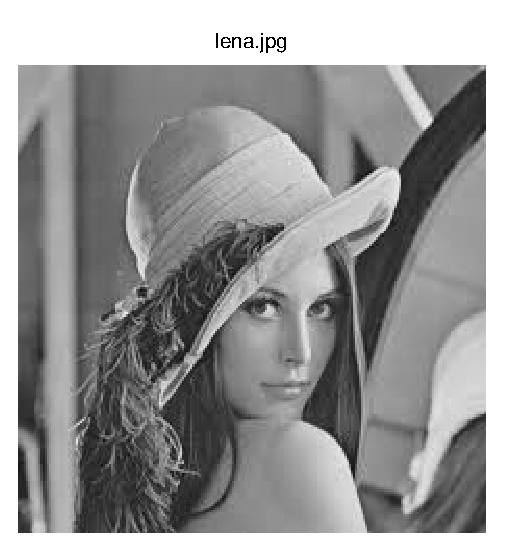
\includegraphics[width=0.3\textwidth]{assignment_1_01.eps}
	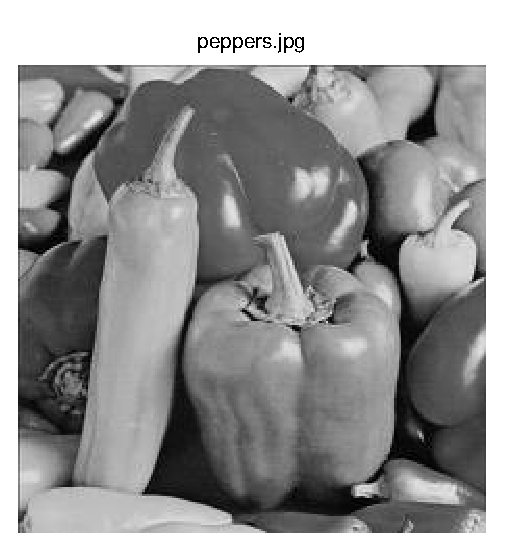
\includegraphics[width=0.3\textwidth]{assignment_1_02.eps}
	\caption{Question 1 (a)}
\end{figure}

\subsection*{Question 1 (b)}

\begin{figure}[!htm]
	\centering
	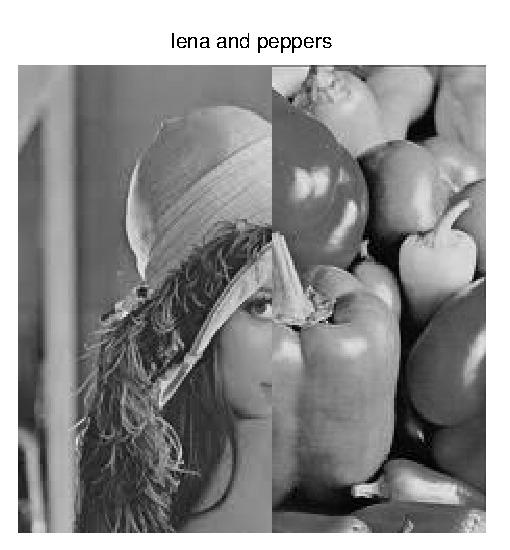
\includegraphics[width=0.4\textwidth]{assignment_1_03.eps}
	\caption{Question 1 (b)}
\end{figure}

\clearpage
\subsection*{Question 2 (a)}

\begin{figure}[!htm]
	\centering
	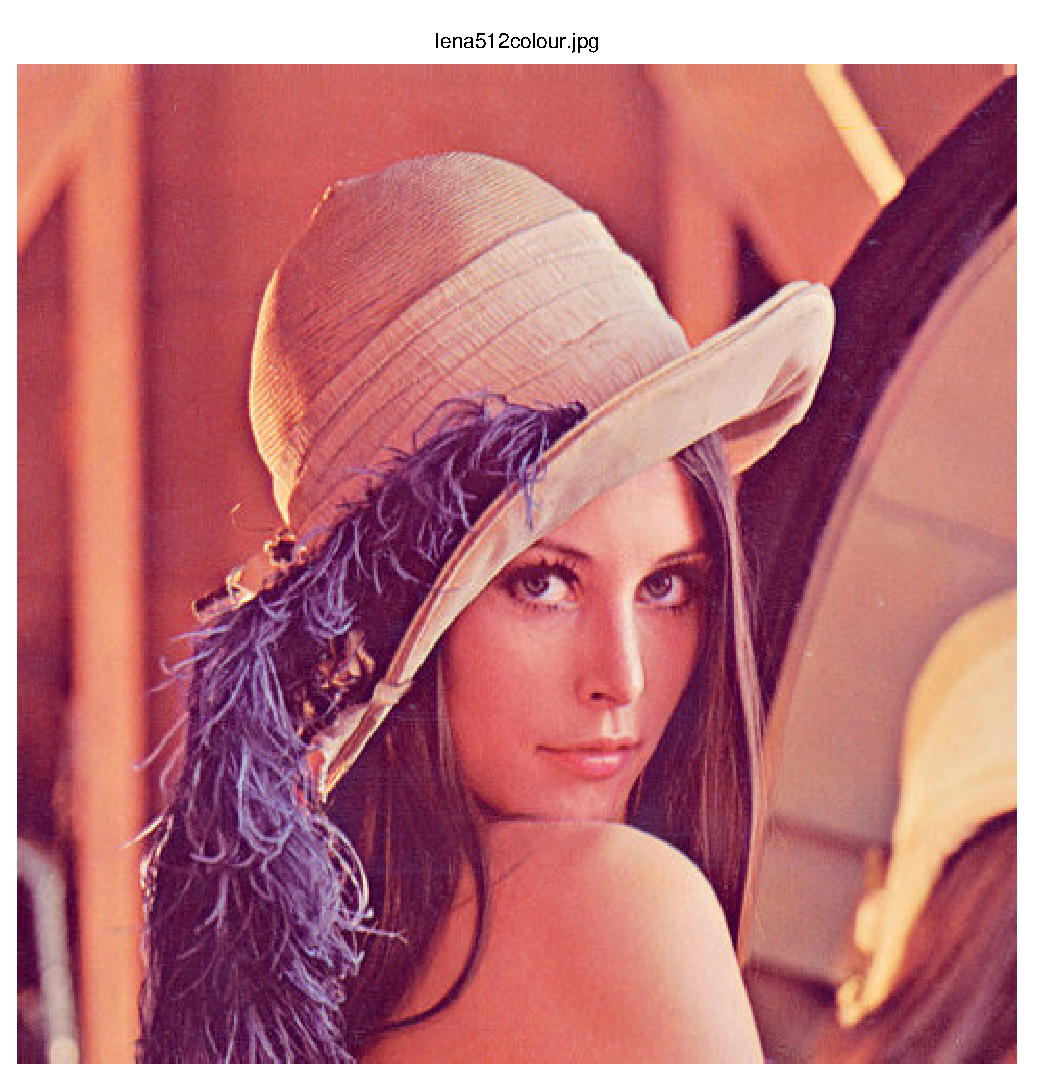
\includegraphics[width=0.6\textwidth]{assignment_1_04.eps}
	\caption{Question 2 (a)}
\end{figure}

\clearpage
\subsection*{Question 2 (b, c)}

\begin{figure}[!htm]
	\centering
	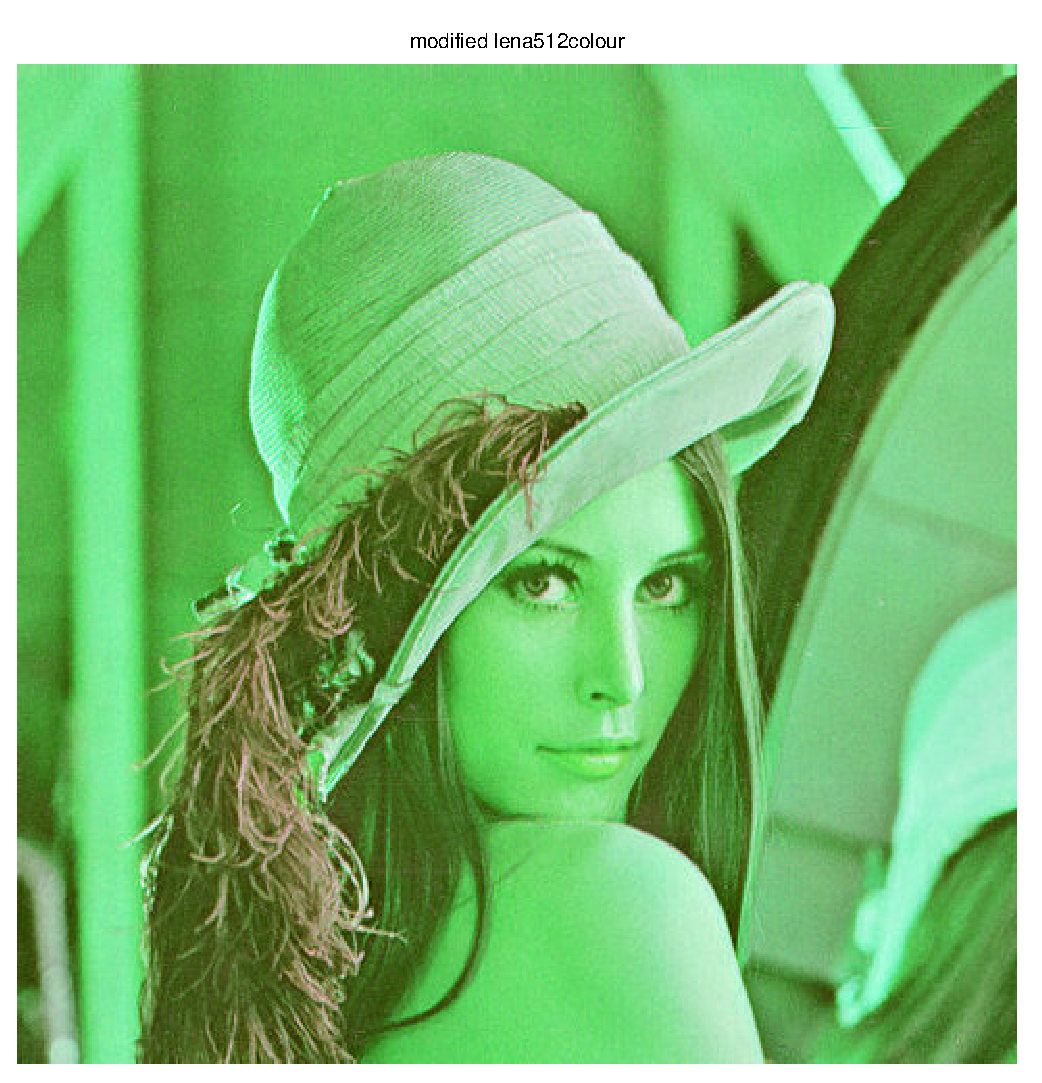
\includegraphics[width=0.6\textwidth]{assignment_1_05.eps}
	\caption{Question 2 (b, c)}
\end{figure}


\clearpage
\appendix

\section{Complete Code}

\begin{Verbatim}[frame=lines, label=Initialization]
clc;
clear;
close all;
\end{Verbatim}

\begin{Verbatim}[frame=lines, label=Question 1 (a)]
% %%%%%%Read image%%%%%%

I1=imread('lena.jpg');
I2=imread('peppers.jpg');

% %%%%%%Show image%%%%%%
% show lena.jpg
figure, imshow(I1);
title('lena.jpg');
% show
figure, imshow(I2);
title('peppers.jpg');
\end{Verbatim}

\begin{Verbatim}[frame=lines, label=Question 1 (b)]
% %%%%%%Construct image A%%%%%%
A=[I1(:,1:122,:), I2(:, 123:end, :)];

% %%%%%%Show image A%%%%%%
figure, imshow(A);
title('lena and peppers');
\end{Verbatim}

\begin{Verbatim}[frame=lines, label=Question 2 (a)]
% %%%%%%Read image%%%%%%

A1=imread('lena512colour.jpg');

% %%%%%%Show image%%%%%%
figure, imshow(A1)
title('lena512colour.jpg');
\end{Verbatim}

\begin{Verbatim}[frame=lines, label={Question 2 (b, c)}]
% %%%%%%Duplicate image%%%%%%
A2=A1;

% %%%%%%Change colour band of A2%%%%%%
A2(:,:,1)=A1(:,:,3);
A2(:,:,2)=A1(:,:,1);
A2(:,:,3)=A1(:,:,2);

%% Question 2 (c)

% %%%%%%Show and save image%%%%%%
figure, imshow(A2);
title('modified lena512colour');

imwrite(A2, 'newlena512colour.jpeg', 'jpeg');
\end{Verbatim}



\end{document}
    
